% 第1章第1节：状态更新与轨迹（递推关系与状态选择；迭代、轨道与不变集合；历史累计与状态扩充）。

\section{状态更新与轨迹}
\label{sec:dds-state-updates}

本节建立全章共用的对象。一条轨迹由四样东西决定：允许出现的状态，按步编号的时间，事先给定的外部输入，以及把当前状态和当前输入变成下一状态的更新规则。把它们分开写清，后面讨论求解、稳定和误差时才知道比较的是什么、哪些量固定不变。

\subsection{递推关系与状态选择}
\label{sec:dds-recurrence-state}

\paragraph{一分钟一步的温度}
回到章首的房间。环境温度固定，$x_n$表示第$n$分钟时房间相对环境的温差，$u_n$表示第$n$分钟内的加热量。模型
\begin{equation}
  x_{n+1}=0.8x_n+u_n
  \label{eq:dds-temperature}
\end{equation}
说：不加热时，温差每分钟保留八成，其余散到环境里；加热则直接补充温差。取$x_0=0$、$u_n=0.4$，逐步代入得到
\[
  \begin{gathered}
  x_1=0.4,\quad x_2=0.72,\quad x_3=0.976,\\
  x_4=1.1808,\quad x_5=1.34464,\quad x_6\approx1.4757.
  \end{gathered}
\]
数列在增长，增量却越来越小，看上去在逼近某个值。

这个值可以从递推式本身读出。若存在不随时间改变的温差$x_*$，它必须满足$x_*=0.8x_*+0.4$，即$x_*=2$。把式~\eqref{eq:dds-temperature}两边同减$2$，
\[
  x_{n+1}-2=0.8x_n+0.4-2=0.8\,(x_n-2).
\]
所以与平衡值的偏差每一步乘以$0.8$：$x_n-2=0.8^n(x_0-2)=-2\times0.8^n$。图~\ref{fig:dds-temperature-trajectory}把三条不同起点的轨迹画在一起：无论从下方还是上方出发，它们都向$2$靠拢；换成对数纵轴后，三条偏差曲线变成斜率相同的平行直线，斜率就是$\ln0.8$。

\begin{figure}[htbp]
  \centering
  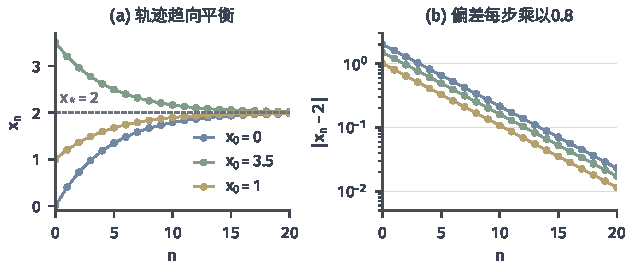
\includegraphics[width=107mm]{figures/03-optimization-evolution-and-signals/02-processes-and-trajectory-evolution/matplotlib/dds-temperature-trajectory/figure.pdf}
  \caption{温度递推$x_{n+1}=0.8x_n+0.4$的轨迹。(a)三个初值$x_0=0,\,1,\,3.5$的前$20$步，虚线为平衡温差$x_*=2$；(b)同三条轨迹的偏差$|x_n-2|$，纵轴取对数。偏差每步乘以$0.8$，在对数坐标中是斜率为$\ln0.8$的平行直线，起点只决定直线的高低。}
  \label{fig:dds-temperature-trajectory}
\end{figure}

这个小计算已经把两个量分开了。平衡位置$x_*=u/(1-0.8)$由系数和输入共同决定：把恒定加热改成$0.5$，平衡升到$2.5$。接近平衡的速度只由系数$0.8$决定：输入改变时，偏差仍然每步乘以$0.8$；系数改成$0.5$，偏差每步减半，接近得快得多。只报告“最终温度”不能说明轨迹，因为同一个终点可以由快慢完全不同的过程到达。

\paragraph{状态应当记住什么}
式~\eqref{eq:dds-temperature}之所以能一步一步算下去，是因为下一时刻的温差只依赖当前温差和当前加热量，过去更早的加热已经全部体现在$x_n$里。这个性质不是变量名称自动带来的，而是模型的假设。假如墙体也会蓄热：同样的室温下，墙体较热时房间散热慢，墙体较冷时散热快，那么只看室温就预测不了下一分钟。

设$h_n$为墙体相对环境的温差，取教学用的扩充模型
\[
  \begin{bmatrix}x_{n+1}\\h_{n+1}\end{bmatrix}
  =\begin{bmatrix}0.8&0.1\\0.1&0.9\end{bmatrix}
   \begin{bmatrix}x_n\\h_n\end{bmatrix}
  +\begin{bmatrix}0.4\\0\end{bmatrix}.
\]
两个初态都有$x_0=0$，加热量也相同，但$h_0=2$给出$x_1=0.6$，$h_0=-2$给出$x_1=0.2$。图~\ref{fig:dds-state-sufficiency}把两条轨迹继续画下去：相同的当前室温对应不同的未来。对这个模型，室温一个坐标不够，必须把$(x_n,h_n)$一起记作状态。

\begin{figure}[htbp]
  \centering
  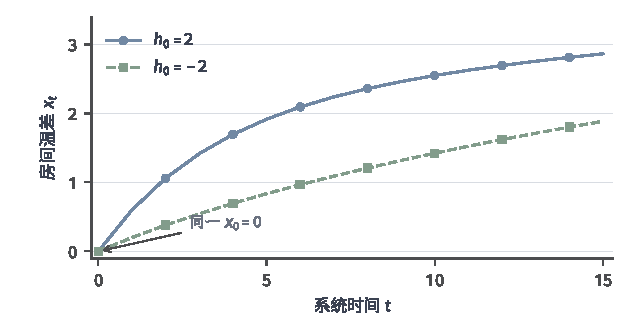
\includegraphics[width=107mm]{figures/00-shared/mathematical-preliminaries-lower/02-dynamical-systems-control-decision-and-games/matplotlib/reader-state-sufficiency/figure.pdf}
  \caption{室温单坐标遗漏墙体蓄热时的预测差异。按正文的双状态教学模型逐步计算，两条曲线的房间初始温差均为$x_0=0$，恒定加热量均为$0.4$；仅墙体初始温差$h_0$分别取$2$与$-2$。相同的当前室温对应不同的后继轨迹，说明状态要按“未来依赖什么”来选。}
  \label{fig:dds-state-sufficiency}
\end{figure}

由此可以给出本章的基本对象。选择状态的标准是：已知当前状态和当前输入，下一状态就被唯一确定，不必再回看更早的历史。

\begin{definition}[离散时间状态模型]
\label{def:dds-state-model}
设$X$为非空集合，称为\term{状态空间}（state space）；$U$为非空集合，称为输入集合。对每个$n\in\mathbb N$给定映射$F_n:X\times U\to X$。对初值$x_0\in X$与输入序列$(u_n)_{n\geq0}\subseteq U$，递推
\begin{equation}
  x_{n+1}=F_n(x_n,u_n),\qquad n=0,1,2,\ldots
  \label{eq:dds-state-model}
\end{equation}
唯一确定序列$(x_n)_{n\geq0}$，称为从$x_0$出发、受输入$(u_n)$驱动的\term{轨迹}（trajectory）。$x_n$称为时刻$n$的\term{状态}（state）。
\end{definition}

定义要求$F_n$的值仍落在$X$中，这是“每一步都有定义”的保证：只要$x_n\in X$，$x_{n+1}$就有意义，归纳下去整条轨迹都有意义。实际建模时，更新公式往往只在某个区域内有意义，比如要开平方根或取对数；这时必须把$X$取成公式能映回自身的集合，或者逐步检查轨迹没有离开公式的定义域。第~\ref{sec:dds-orbits-invariant}小节会用不变区间系统地处理这件事。

\paragraph{高阶递推改写为一阶向量递推}
状态选择的另一种常见情形来自高阶递推。用带动量的梯度下降最小化$f(\theta)=\theta^2/2$，步长$\eta$、动量系数$\beta$时，参数按
\[
  \theta_{n+1}=\theta_n-\eta\theta_n+\beta(\theta_n-\theta_{n-1})
\]
更新。取$\eta=0.5$、$\beta=0.4$，得到二阶递推
\begin{equation}
  \theta_{n+1}=0.9\,\theta_n-0.4\,\theta_{n-1}.
  \label{eq:dds-heavy-ball}
\end{equation}
只知道$\theta_n$不能算出$\theta_{n+1}$：$\theta_n=1$时，$\theta_{n-1}=1$给出$0.5$，$\theta_{n-1}=0$给出$0.9$。动量项记住了“上一步走了多远”，这正是当前参数值没有包含的信息。

办法是把需要的历史并进状态。令$\bm z_n=(\theta_n,\theta_{n-1})^{\top}\in\mathbb R^2$，则
\begin{equation}
  \bm z_{n+1}=\begin{bmatrix}\theta_{n+1}\\ \theta_n\end{bmatrix}
  =\begin{bmatrix}0.9&-0.4\\1&0\end{bmatrix}\bm z_n .
  \label{eq:dds-heavy-ball-state}
\end{equation}
第一行就是原递推，第二行只是把$\theta_n$抄到下一个状态的第二个位置（图~\ref{fig:dds-state-augmentation}）。初值需要两个数$(\theta_0,\theta_{-1})$，这与二阶递推需要两个初始条件一致。同样的做法适用于任意$k$阶递推$x_{n+1}=G(x_n,\ldots,x_{n-k+1},u_n)$：取最近$k$个值组成的向量为状态，状态空间变成$X^k$，更新仍是一阶的。

\begin{figure}[htbp]
  \centering
  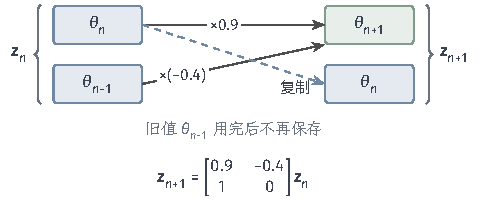
\includegraphics[width=90mm]{figures/03-optimization-evolution-and-signals/02-processes-and-trajectory-evolution/tikz/dds-state-augmentation/figure.pdf}
  \caption{二阶递推$\theta_{n+1}=0.9\theta_n-0.4\theta_{n-1}$的状态扩充。状态$\bm z_n$同时保存$\theta_n$与$\theta_{n-1}$；一步更新用两者算出$\theta_{n+1}$，并把$\theta_n$复制到新状态的第二个位置，最旧的值随之丢弃。整个操作是一次$2\times2$矩阵乘法。}
  \label{fig:dds-state-augmentation}
\end{figure}

这个例子后面还会出现：第~\ref{sec:dds-constant-coefficient}小节将看到，矩阵~\eqref{eq:dds-heavy-ball-state}有一对复特征值，所以动量迭代会一边振荡一边收敛。

\paragraph{自治、线性与时变}
有了一般形式，就可以按更新规则的结构给系统分类。若$F_n=F$不依赖$n$，且没有输入或输入恒定，系统写成$x_{n+1}=F(x_n)$，称为\term{自治}（autonomous）系统；否则称为非自治系统。给定一条输入序列后，令$F_n^{u}(x)=F_n(x,u_n)$，系统就成为只含状态的非自治递推$x_{n+1}=F_n^{u}(x_n)$。本章讨论稳定性时主要使用自治形式，恒定输入的情形通过平移平衡点化归过来。

另一种分类看$F_n$是否线性。当$X=\mathbb R^d$、$U=\mathbb R^m$时，\term{线性系统}（linear system）指
\begin{equation}
  \bm x_{n+1}=\bm A_n\bm x_n+\bm B_n\bm u_n,\qquad
  \bm A_n\in\mathbb R^{d\times d},\ \bm B_n\in\mathbb R^{d\times m},
  \label{eq:dds-linear-system}
\end{equation}
它关于状态与输入的联合变量$(\bm x,\bm u)$是线性映射。系数矩阵不随$n$变化时称为时不变或定常，否则称为时变。线性与时变是两项相互独立的性质：$x_{n+1}=0.8x_n+\sin n$是线性时变的，$x_{n+1}=x_n^2$是非线性时不变的。“离散时间”又是第三项独立的性质，它只说明时间按步编号。

线性有两个容易混淆的地方。第一，固定一条非零输入后，$\bm x\mapsto\bm A\bm x+\bm B\bm u_n$关于状态是\term{仿射映射}（affine map），不是线性映射：温度模型~\eqref{eq:dds-temperature}在$u_n=0.4$时，从$x_0=0$与$x_0=1$出发的第一步分别是$0.4$和$1.2$，而从$x_0=0+1$出发的第一步是$1.2$，不等于$0.4+1.2$。叠加原理对初值与输入一起成立，对初值单独不成立。第二，“系数乘状态”的外形不能保证线性。$x_{n+1}=(0.5+0.1x_n^2)\,x_n$看上去像系数$0.5+0.1x_n^2$乘以$x_n$，但系数本身依赖状态，把初值加倍后下一步并不加倍：$x_0=1$给出$0.6$，$x_0=2$给出$1.8$。

\subsection{迭代、轨道与不变集合}
\label{sec:dds-orbits-invariant}

\paragraph{多步映射与前向轨道}
自治系统$x_{n+1}=F(x_n)$的多步状态由映射复合给出。记$F^0=\operatorname{id}$，$F^{n}=F\circ F^{n-1}$，则$x_n=F^n(x_0)$。本章中映射的上标$F^n$一律表示$n$次复合，而不是函数值的$n$次幂；对线性映射$\bm x\mapsto\bm A\bm x$，$n$次复合恰好是矩阵幂$\bm A^n$，两种读法一致。复合满足
\[
  F^{m+n}=F^m\circ F^n,\qquad m,n\geq0,
\]
即走$m+n$步等于先走$n$步、再从到达的位置走$m$步。这条性质说明状态确实“概括了过去”：从$x_n$重新开始计算，与从$x_0$一口气算下去得到同样的未来。

非自治系统也有多步映射，只是要按时间排序：
\[
  x_n=(F_{n-1}\circ\cdots\circ F_1\circ F_0)(x_0),
\]
较晚的更新写在左边，因为它作用在较早更新的结果上。顺序不能交换：$F_0(x)=2x$、$F_1(x)=x+1$时，从$x_0=1$出发得$F_1(F_0(1))=3$，若误写成$F_0(F_1(1))$则得到$4$。

\begin{definition}[轨道与不变集合]
\label{def:dds-orbit-invariant}
设$F:X\to X$。点$x_0\in X$的\term{轨道}（orbit）指序列$(F^n(x_0))_{n\geq0}$，其取值集合$\{F^n(x_0):n\geq0\}$称为前向轨道集合。若子集$S\subseteq X$满足$F(S)\subseteq S$，称$S$为\term{正向不变集}（positively invariant set）；若$F(S)=S$，称$S$为\term{不变集}（invariant set）。
\end{definition}

正向不变集的意思是“进得来、出不去”：若$x_0\in S$，归纳可知全部$x_n\in S$。不变集还多要求一件事：$S$中每一点都有$S$中的前像，因而可以在$S$内往过去追溯。区分二者在第~\ref{sec:dds-limit-sets}小节讨论极限集合时会用到。

递推在每一步都有定义，只能保证有限长的轨道可以算出，不能保证轨道有界或收敛。$x_{n+1}=2x_n$对一切实数有定义，轨道$2^nx_0$却在$x_0\neq0$时无界；长期行为是需要另外证明的性质，第~\ref{sec:dynamical-stability-sensitivity}节和第~\ref{sec:dds-nonlinear-long-term}节专门处理它。

\paragraph{不变区间与持续运行}
现在处理公式只在部分区域有意义的情形。考察
\begin{equation}
  x_{n+1}=\sqrt{2-x_n},
  \label{eq:dds-sqrt-map}
\end{equation}
它只在$x_n\leq2$时有定义。从$x_0=-7$出发，$x_1=3$，下一步就要对$-1$开平方，递推中断。要让递推永远运行，需要找一个区间$I$，使公式在$I$上有定义且把$I$映回$I$。

取$I=[0,2]$。对$x\in[0,2]$，有$0\leq2-x\leq2$，所以$\sqrt{2-x}\in[0,\sqrt2]\subseteq[0,2]$。于是$F([0,2])\subseteq[0,2]$，$[0,2]$是正向不变区间，从其中任何一点出发的轨道都永远有定义。区间还可以放大到$[-2,2]$：其中的$x$满足$0\leq2-x\leq4$，一步之后落进$[0,2]$，此后留在那里。再大就不行了，$x_0<-2$使$x_1=\sqrt{2-x_0}>2$，第二步失去定义。所以“轨道永远有定义”的初值恰好组成$[-2,2]$，这个集合要由映射本身算出来，不能从公式的定义域$(-\infty,2]$直接读出。

同样的检查对本章的主要非线性例子必不可少。\term{Logistic映射}（logistic map）
\begin{equation}
  F_r(x)=r\,x(1-x),\qquad r\geq0,
  \label{eq:dds-logistic}
\end{equation}
是种群模型的离散版本：$x$表示种群占环境容量的比例，$rx$是无约束时的增长，$1-x$表示拥挤造成的抑制。$F_r$在$x=1/2$处取最大值$r/4$，在$[0,1]$上非负。所以当$0\leq r\leq4$时$F_r([0,1])\subseteq[0,r/4]\subseteq[0,1]$，$[0,1]$是正向不变区间，比例解释始终成立。当$r>4$时，靠近$1/2$的点会被送出$[0,1]$：$r=4.5$、$x_0=0.5$给出$x_1=1.125$、$x_2\approx-0.633$、$x_3\approx-4.65$、$x_4\approx-118$，此后迅速趋于$-\infty$，“比例”的含义早已失效。

\paragraph{正向迭代与逆向恢复}
动力系统沿时间向前走，自然要问能否向后走：已知现在，能否唯一恢复过去？若$F:X\to X$是双射，答案是肯定的，$F^{-n}=(F^{-1})^n$把轨道延伸到负时间。线性映射$\bm x\mapsto\bm A\bm x$可逆当且仅当$\bm A$可逆。

更新不可逆时，向后追溯会遇到两种障碍。一是多个过去汇合到同一个现在：$F(x)=x^2$把$0.8$和$-0.8$都映到$0.64$（图~\ref{fig:dds-noninvertible-merge}），站在$x_1=0.64$处无法判断来自哪一边。二是有的状态根本没有前像：负数不是任何实数的平方，所以$x_1=-0.5$不可能由这个更新产生。Logistic映射$F_4$同样不可逆，因为$F_4(x)=F_4(1-x)$。线性的例子是$\bm A=\operatorname{diag}(1,0)$，它把第二个坐标清零，所有横坐标相同的初值一步之后都汇合到同一点。

\begin{figure}[htbp]
  \centering
  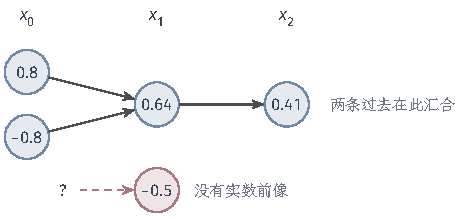
\includegraphics[width=86mm]{figures/03-optimization-evolution-and-signals/02-processes-and-trajectory-evolution/tikz/dds-noninvertible-merge/figure.pdf}
  \caption{不可逆更新$F(x)=x^2$使不同的过去汇合。$x_0=0.8$与$x_0=-0.8$在第一步都到达$0.64$，此后轨道完全相同（$0.64^2\approx0.41$）。负数$-0.5$没有实数前像，因此不能出现在任何轨道的第一步之后。}
  \label{fig:dds-noninvertible-merge}
\end{figure}

这说明离散动力系统的时间方向通常不对称：未来由现在唯一决定，过去却不一定。后面研究长期行为时只使用正向迭代；凡需要往回追溯的地方，例如不变集要求每点都有前像，都会单独说明。

\subsection{历史累计与状态扩充}
\label{sec:dds-history-augmentation}

前两小节从“已有的更新规则需要什么状态”出发。这一小节反过来：先确定希望保留历史的哪些方面，再问能否构造一个有限维状态，让它带着这些信息逐步更新。

\paragraph{有限窗口的累计}
设输入$u_n$是每分钟的加热量，我们想随时知道最近三分钟的总加热量$s_n=u_n+u_{n-1}+u_{n-2}$。能否只用$s_{n-1}$和新输入$u_n$更新$s_n$？写出差就知道不行：
\[
  s_n=s_{n-1}+u_n-u_{n-3},
\]
右边需要即将移出窗口的$u_{n-3}$，它不在$s_{n-1}$中。总和这一个数丢掉了窗口内部的排列，而移出窗口时恰好需要知道最旧的那一项。

闭合的办法是保存整个窗口。令$\bm w_n=(u_n,u_{n-1},u_{n-2})^{\top}$，则
\[
  \bm w_{n+1}=\begin{bmatrix}0&0&0\\1&0&0\\0&1&0\end{bmatrix}\bm w_n+\begin{bmatrix}1\\0\\0\end{bmatrix}u_{n+1},
  \qquad s_n=(1,1,1)\,\bm w_n.
\]
这又是一个线性系统，和图~\ref{fig:dds-state-augmentation}的移位结构相同。代价是维数等于窗口长度$k$：存储和每步计算都随$k$线性增长，窗口取一小时、每秒一个读数时，状态就有$3600$个坐标。

\paragraph{有限统计量未必恢复历史}
若不在乎精确的窗口，而只要一个随时间淡化的平均，就可以用一个数完成闭合更新。\term{指数移动平均}（exponential moving average，EMA）取
\begin{equation}
  m_n=(1-\alpha)\,m_{n-1}+\alpha\,u_n,\qquad 0<\alpha\leq1,
  \label{eq:dds-ema}
\end{equation}
状态只有$m_n$一个坐标，却综合了全部历史：第~\ref{sec:dds-constant-coefficient}小节会把它展开成按$(1-\alpha)^k$衰减的加权和。

一个统计量能闭合地更新，并不意味着它保存了全部有用的历史。

\begin{example}[相同的平均、不同的历史]
\label{ex:dds-ema-insufficient}
取$\alpha=0.5$、$m_0=0$。历史$(u_1,u_2)=(2,0)$给出$m_1=1$、$m_2=0.5$；历史$(0,1)$给出$m_1=0$、$m_2=0.5$。两段历史的EMA相同，此后输入相同则EMA永远相同；但“最近两分钟的总加热量”分别是$2$和$1$，无法从$m_2$读出。
\end{example}

所以状态是否“足够”，取决于我们要预测的是哪一个未来量：$m_n$对它自己的未来是充分的，对窗口总和却不充分。

\paragraph{加权历史的有限基表示}
能不能既只用少数几个坐标，又保留比平均值更丰富的历史形状？一种思路是把整段历史看成一个函数，用少数几个基函数去逼近它，再把展开系数当作状态。离散时间里有一个可以完全算清楚的例子。固定$0<a<1$，定义按距今步数加权的两个矩
\[
  S_0(n)=\sum_{j\leq n}a^{\,n-j}u_j,\qquad
  S_1(n)=\sum_{j\leq n}a^{\,n-j}(n-j)\,u_j,
\]
其中$j$取遍已经发生的时刻。$S_0$是指数加权的总量，$S_1$还按“过去了多久”再加权一次，于是能区分输入集中在近期还是远期。

这两个矩可以闭合地更新。$S_0$的递推$S_0(n)=aS_0(n-1)+u_n$与EMA同型。对$S_1$，把$j=n$的项（权重为$0$）去掉，再把$n-j$写成$(n-1-j)+1$：
\[
  S_1(n)=\sum_{j\leq n-1}a\cdot a^{\,n-1-j}\bigl((n-1-j)+1\bigr)u_j
  =a\bigl(S_1(n-1)+S_0(n-1)\bigr).
\]
合起来，$\bm S(n)=(S_0(n),S_1(n))^{\top}$满足线性递推
\begin{equation}
  \bm S(n)=a\begin{bmatrix}1&0\\1&1\end{bmatrix}\bm S(n-1)+\begin{bmatrix}1\\0\end{bmatrix}u_n .
  \label{eq:dds-moment-state}
\end{equation}
两个坐标足以支撑一个有用的读出：在权重$a^{\,n-j}$下用直线$c_0+c_1(j-n)$拟合历史输入，加权最小二乘的正规方程只涉及两类量：权重的和$\sum_k a^k$、$\sum_k ka^k$、$\sum_k k^2a^k$（只依赖$a$与已经过去的步数，与输入无关），以及数据矩$S_0(n)$、$S_1(n)$。所以拟合直线的截距和斜率都是状态的函数。图~\ref{fig:dds-history-moments}画出一段带噪输入、所用的指数权重，以及仅凭$\bm S(n)$读出的局部直线。

\begin{figure}[htbp]
  \centering
  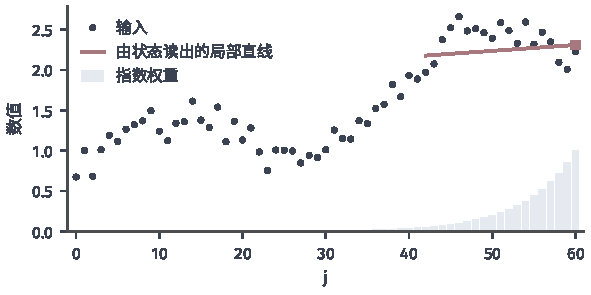
\includegraphics[width=100mm]{figures/03-optimization-evolution-and-signals/02-processes-and-trajectory-evolution/matplotlib/dds-history-moments/figure.pdf}
  \caption{用两个指数加权矩概括历史。黑点为教学用输入$u_j=0.6+0.03j+0.5\sin(j/6)+$噪声（固定随机种子），浅蓝柱为$n=60$时的权重$a^{\,n-j}$，$a=0.85$。红线是只用状态$\bm S(60)=(S_0,S_1)$算出的加权最小二乘直线，方块为其在当前时刻的值。权重集中在最近约十几步，远处的起伏几乎不影响状态。}
  \label{fig:dds-history-moments}
\end{figure}

与均匀窗口对照，可以看出闭合的来源。均匀窗口在左端硬性截断，移出窗口的旧输入必须单独记住；指数权重每步整体乘以$a$，旧输入的影响自动变小，不需要知道它具体是哪一项。所以有限个特征能否自行演化，取决于权重与基的配合，而不是特征个数。

高阶多项式投影（high-order polynomial projection operators，HiPPO）框架系统地发展了这一思路：在连续时间里，选定一个历史测度和一组正交多项式，把到当前为止的输入投影到前$d$个多项式上，并推导投影系数满足的线性方程\scite{gu2020hippo}。不同的测度对应不同的遗忘方式，例如固定长度的滑动窗口或随时间拉长的均匀窗口。连续形式及其离散化留到第~\ref{chap:ordinary-differential-equations}章结合线性状态方程讨论。这里需要分清两项检查：投影误差回答“状态能多准确地重建历史”，状态充分性回答“状态能否决定我们关心的未来”。前者小不保证后者成立，前面EMA的例子已经说明，一个对自身未来充分的状态，仍可能丢掉另一项未来量所需的历史。
